\documentclass[landscape]{article}
\usepackage[utf8]{inputenc}

\usepackage{microtype}

\usepackage{graphicx}

\usepackage{color}

\usepackage{tikz}

\usepackage{pifont}

\usepackage{fourier-orns}

\usepackage{calculator}
% Card Arena v0.1 Colors

% Character colours
\definecolor{red}{RGB}{244,56,36}
\definecolor{blue}{RGB}{36,45,140}
\definecolor{purple}{RGB}{128,0,128}
\definecolor{green}{RGB}{63,165,56}
\definecolor{orange}{RGB}{216,128,43}
\definecolor{teal}{RGB}{51,179,198}
\definecolor{yellow}{RGB}{244,226,66}
\definecolor{brown}{RGB}{145,95,39}

\definecolor{water}{RGB}{00,119,190}
\definecolor{forest}{RGB}{65,117,5}
\definecolor{city}{RGB}{181,114,4}
\usetikzlibrary{shapes}

\pgfmathsetmacro{\hexSize}{2.5}
\pgfmathsetmacro{\hexIconSize}{0.5*\hexSize}
\pgfmathsetmacro{\tinyhexSize}{0.2*\hexSize}
\pgfmathsetmacro{\tinyhexIconSize}{0.5*\tinyhexSize}
% In the pointy orientation, a hexagon has:
% width w = sin(60) * size
% The horizontal distance between adjacent hexagon centers is w.	
\pgfmathsetmacro{\hdist}{sin(60)*\hexSize}

\tikzset{
	hexa/.style= {
		shape=regular polygon,
		regular polygon sides=6,
		minimum size=\hexSize cm, draw,
		inner sep=0,anchor=south,
		fill=lightgray!80!white,
		rotate=30 % looks quite interesting without this
	}
}
\tikzset{
	flathexa/.style= {
		shape=regular polygon,
		regular polygon sides=6,
		minimum size=\hexSize cm, draw,
		inner sep=0,anchor=south,
		fill=lightgray!80!white
		% rotate=30 % looks quite interesting without this
	}
}
\tikzset{
	tinyhexa/.style= {
		shape=regular polygon,
		regular polygon sides=6,
		minimum size=\tinyhexSize cm, draw,
		inner sep=0,anchor=south,
		fill=lightgray!80!white
		% rotate=30 % looks quite interesting without this
	}
}

\usetikzlibrary{shapes}

\begin{document}
\begin{center}
\pagestyle{empty}

% Water
\foreach \j in {0,...,5}{%
\begin{tikzpicture}
	\node[hexa,fill=water] at (0,0) {
		
\includegraphics[width=\hexIconSize cm]{icons/water_white.png}
	};
\end{tikzpicture}
}

% Forest
\foreach \j in {0,...,15}{%
\begin{tikzpicture}
	\node[hexa,fill=forest] at (0,0) {
		
\includegraphics[width=\hexIconSize cm]{icons/leaf_white.png}
	};
\end{tikzpicture}
}

% City
\foreach \j in {0,...,5}{%
\begin{tikzpicture}
	\node[hexa,fill=city] at (0,0) {
		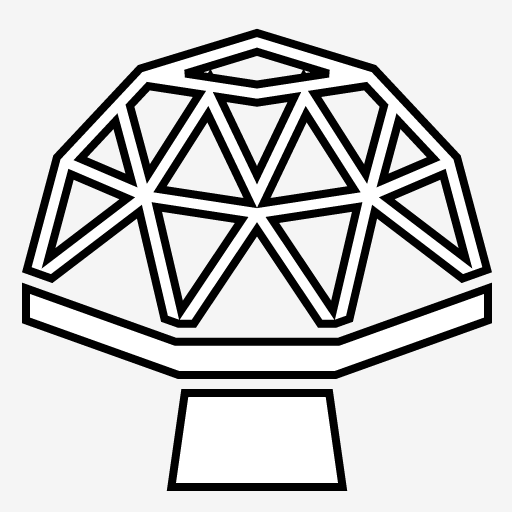
\includegraphics[width=\hexIconSize cm]{icons/city_white.png}
	};
\end{tikzpicture}
}


\end{center}
\end{document}
